\begin{frame}{Sistema Solare e scenario core accretion}
\begin{columns}[T]
	\begin{column}{0.45\textwidth}
	\begin{itemize}
			\item Arricchimento metalli
			\item Oggetti pi\'u antichi hanno et\'a del Sole %($\Omega\tau_{cool}\gg1$): 
			\item numerosa popolazione corpi minori
		\end{itemize}
	\end{column}
	\begin{column}{0.54\textwidth}
		\begin{table}[!ht]
			\begin{flushleft}
\begin{minipage}{.25\linewidth}
	\begin{tabular}{@{}|ccc|@{}}
		\hline
		&\parbox{1.5cm}{Jupiter $317.8\mearth{}$}&\parbox{1.5cm}{Saturn $95.1\mearth{}$}\\
		$M_c$&$0-11\mearth{}$&$9-22\mearth{}$\\
		\hline
		$M_Z$&$1-39\mearth{}$&$1-8\mearth{}$\\
		\hline
		$M_Z^{tot}$&$8-39\mearth{}$&$13-28\mearth{}$\\
		\hline
		$Z/Z_{\odot}$&$1-6$&$6-14$\\
		\hline
	\end{tabular}
\end{minipage}%

\vspace{3mm}
			
			\begin{minipage}{.25\linewidth}
				\centering
				\begin{tabular}{@{}|ccc|@{}}
					\hline
					&\parbox{1.5cm}{Uranus $14.5\mearth{}$}&\parbox{1.5cm}{Neptune $17.1\mearth{}$}\\
					\hline
					$M_{rock}$&$3.7\mearth{}$&$4.2\mearth{}$\\
					\hline
					$M_{ice}$&$9.3\mearth{}$&$10.7\mearth{}$\\
					\hline
					$M_{H/He}$&$1.5\mearth{}$&$2.2\mearth{}$\\
					\hline
				\end{tabular}
			\end{minipage}
					\end{flushleft}
			\caption{Da \cite{baraffe2009physical}.}\label{tab:JSUNcomp}
		\end{table}
	\end{column}
\end{columns}
\end{frame}

\begin{wordonframe}{''ruoli sistema solare'' e intro CA}
[Il sistema solare per primo \'e stato il banco di prova delle teorie di formazione di sistemi planetari: loscenario di core accretion trova giustificazione in alcune caratteristiche del sistema solare e da quest'ultimo \'e possibile stimare in maniera quantitativa la massa del disco protoplanetario da cui ha avuto origine]

I meteoriti pi\'u antichi hanno et\'a compatibile con et\'a del sole quindi \'e plausibile che si siano formati per primi e nello scenario CA trovano collocazione naturale il resto dei corpi minori.
La composizione di giove, saturno e dei pianeti ghiacciati mostra un sostanzioso arricchimento di metalli rispetto al sole: questo sarebbe ovvia conseguenza dell'accrescimento di gas su core solido.

\end{wordonframe}

\begin{frame}{Minimum mass solar nebula}
\begin{columns}[T]
	\begin{column}{0.45\textwidth}
\begin{itemize}
	\item Massa prevista nei modelli GI due ordini di grandezza superiore a MMSN ($Q\gg1$)
\end{itemize}
	\end{column}
	\begin{column}{0.54\textwidth}
			\begin{figure}[!ht]
			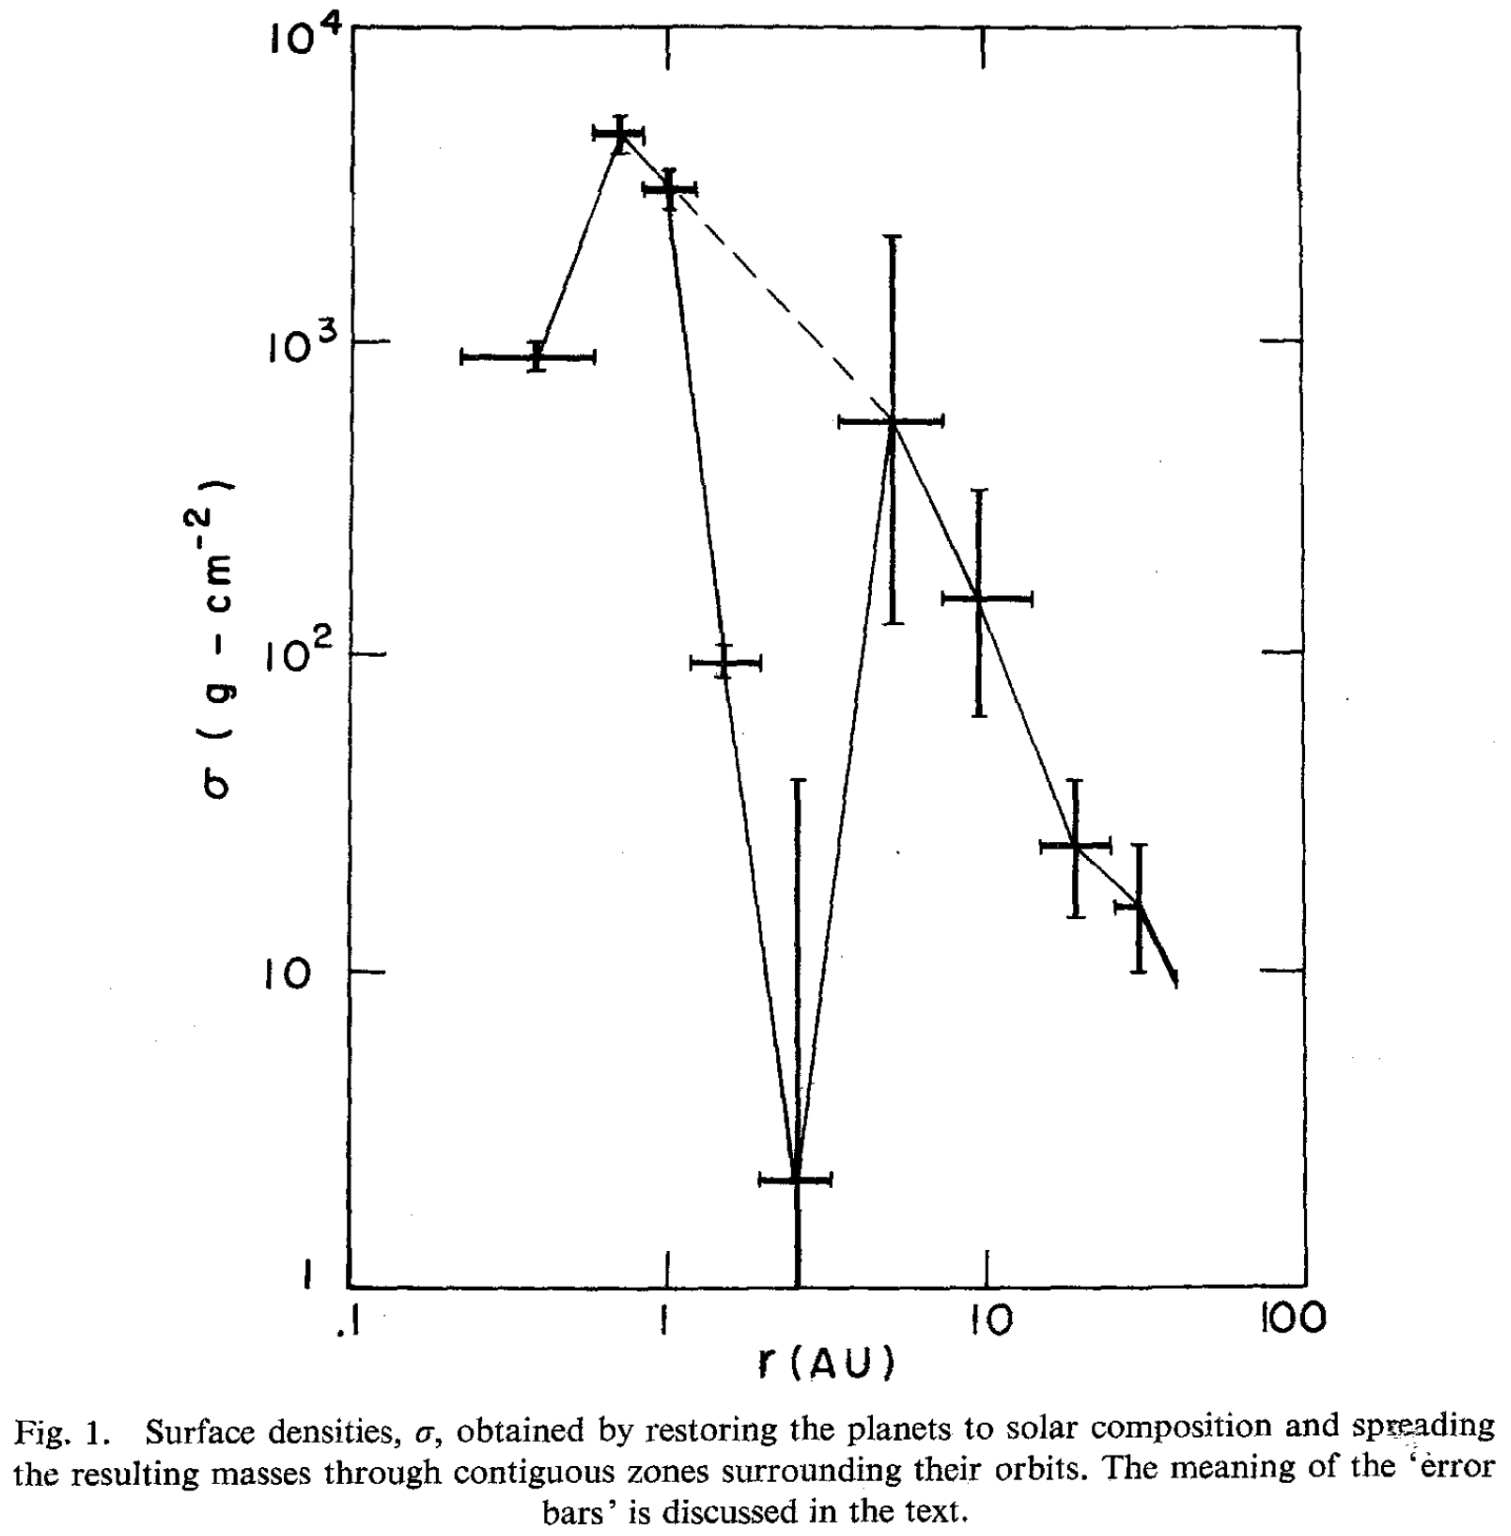
\includegraphics[trim={0cm 5cm 0 0cm},clip, width=0.99\textwidth]{Snebuladensity}
			\caption{Da \cite{weidenschilling1977distribution}.}\label{fig:Snebuladensity}
		\end{figure}
	\end{column}
\end{columns}
\end{frame}

\begin{wordonframe}{Core accretion e MMSN}

Inoltre \'e possibile determinare dalla configurazione attuale,aggiungendo la massa di H/He per ripristinare composizione solare, una stima inferiore della massa iniziale 
\begin{align*}
&\Sigma\propto r\expy{-3/2}
&M\approx0.02\msun{}
\end{align*}

\end{wordonframe}

\begin{frame}{Survey: HARPS}
\begin{figure}[!ht]
	\centering
	\begin{subfigure}[b]{0.37\textwidth}
		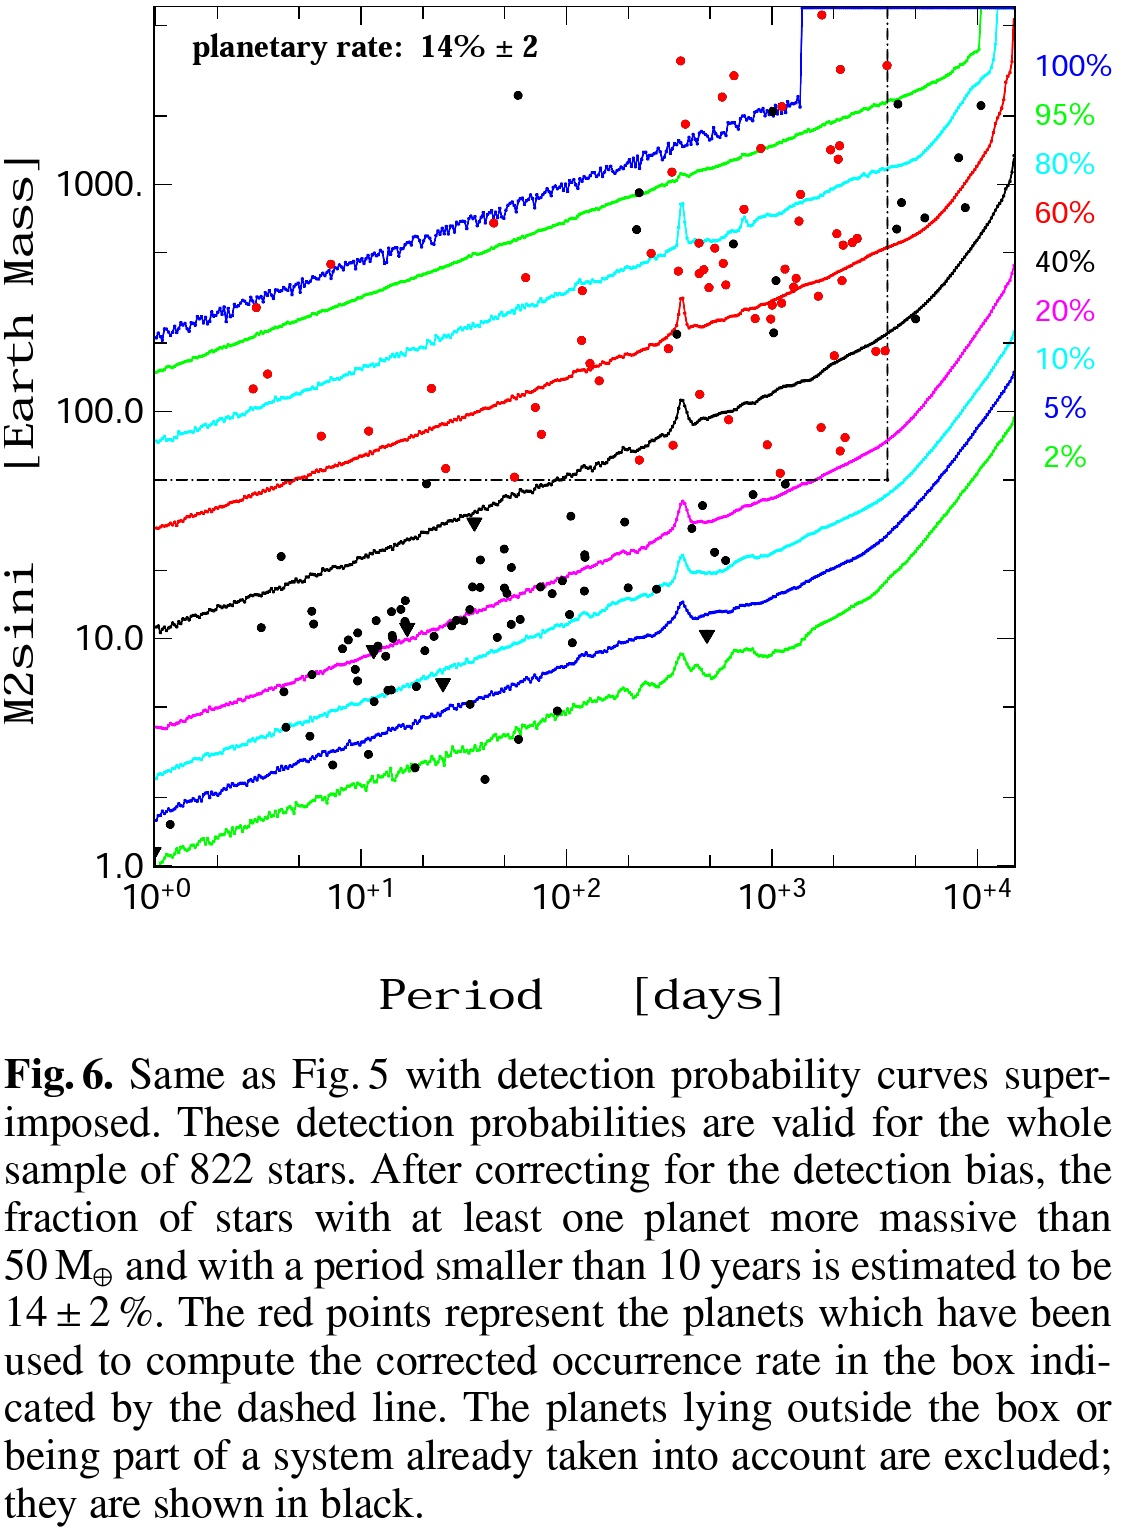
\includegraphics[trim={0cm 17cm 1cm 0},clip, width=0.99\textwidth]{PMfreq-e23}\label{fig:PMfreq-e23}
	\end{subfigure}
	~
	\begin{subfigure}[b]{0.37\textwidth}
		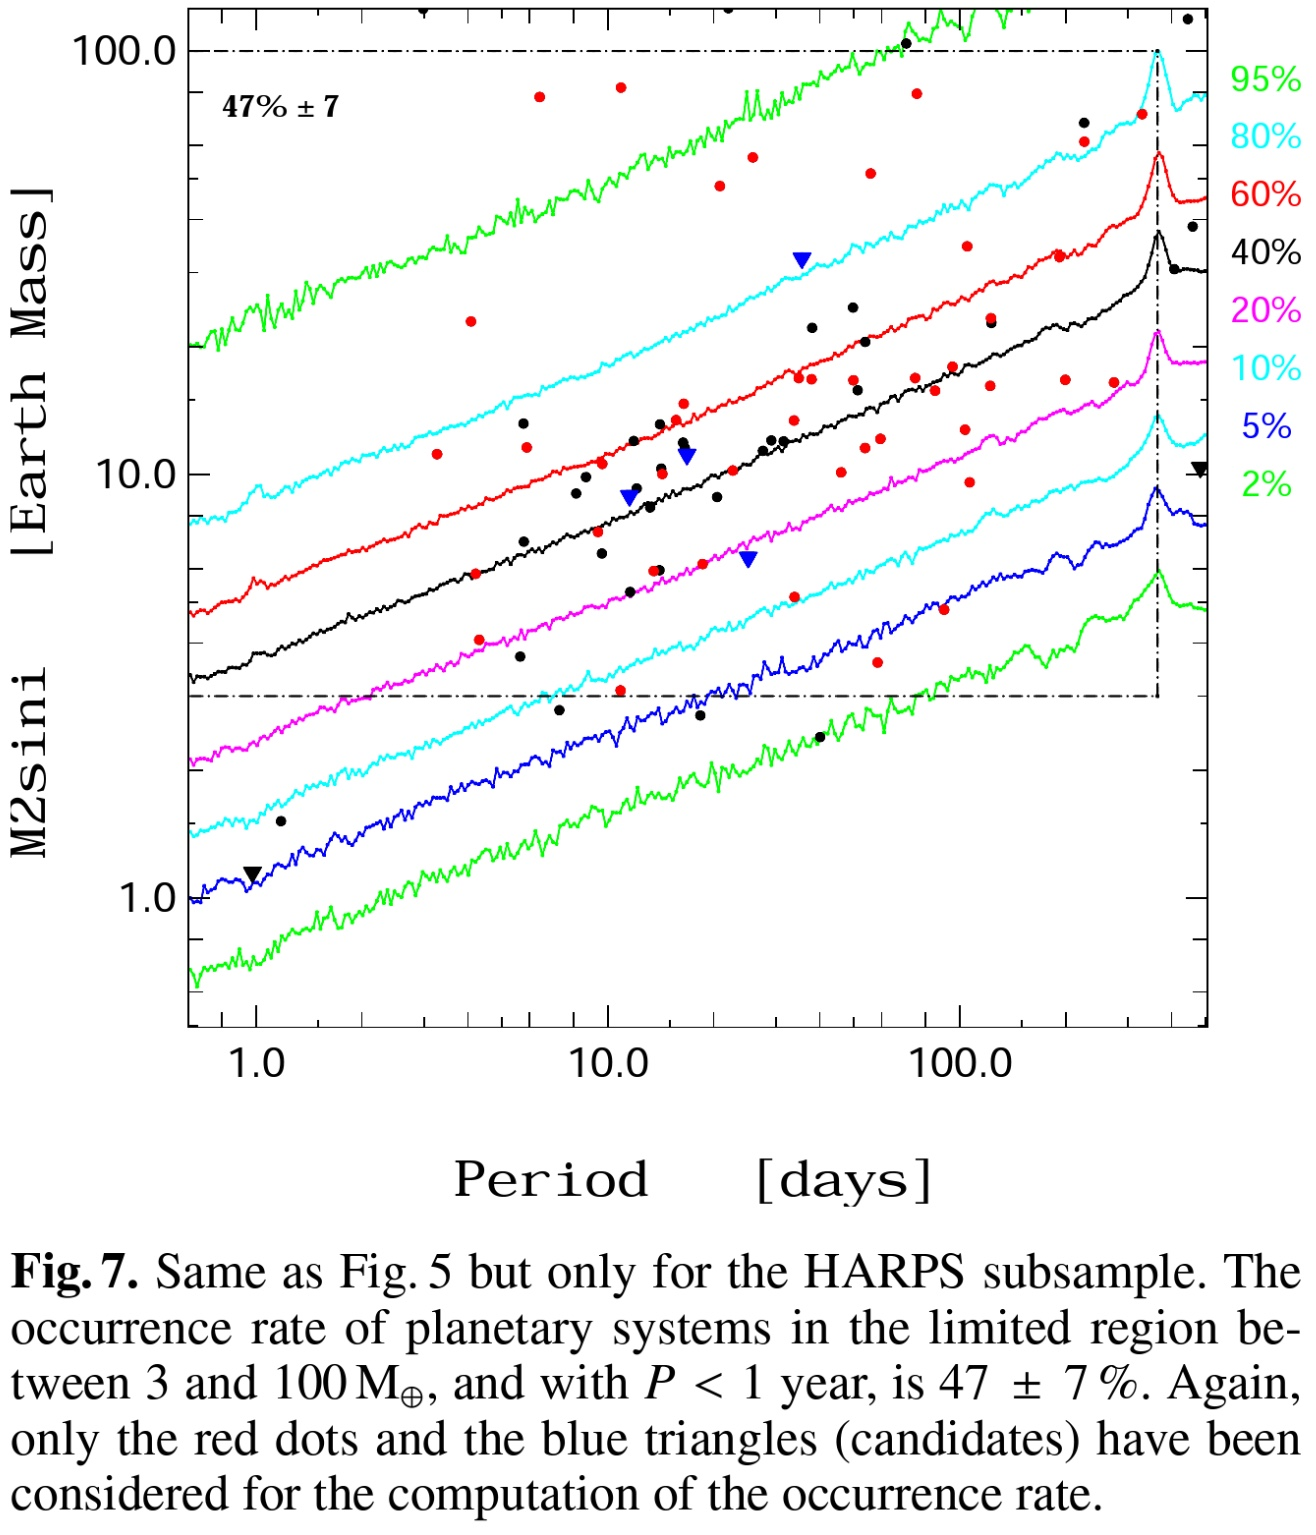
\includegraphics[trim={0cm 10cm 0 0},clip, width=0.99\textwidth]{PMfreq-e12}\label{fig:PMfreq-e12}
	\end{subfigure}%
	
	\begin{subfigure}[b]{0.38\textwidth}
		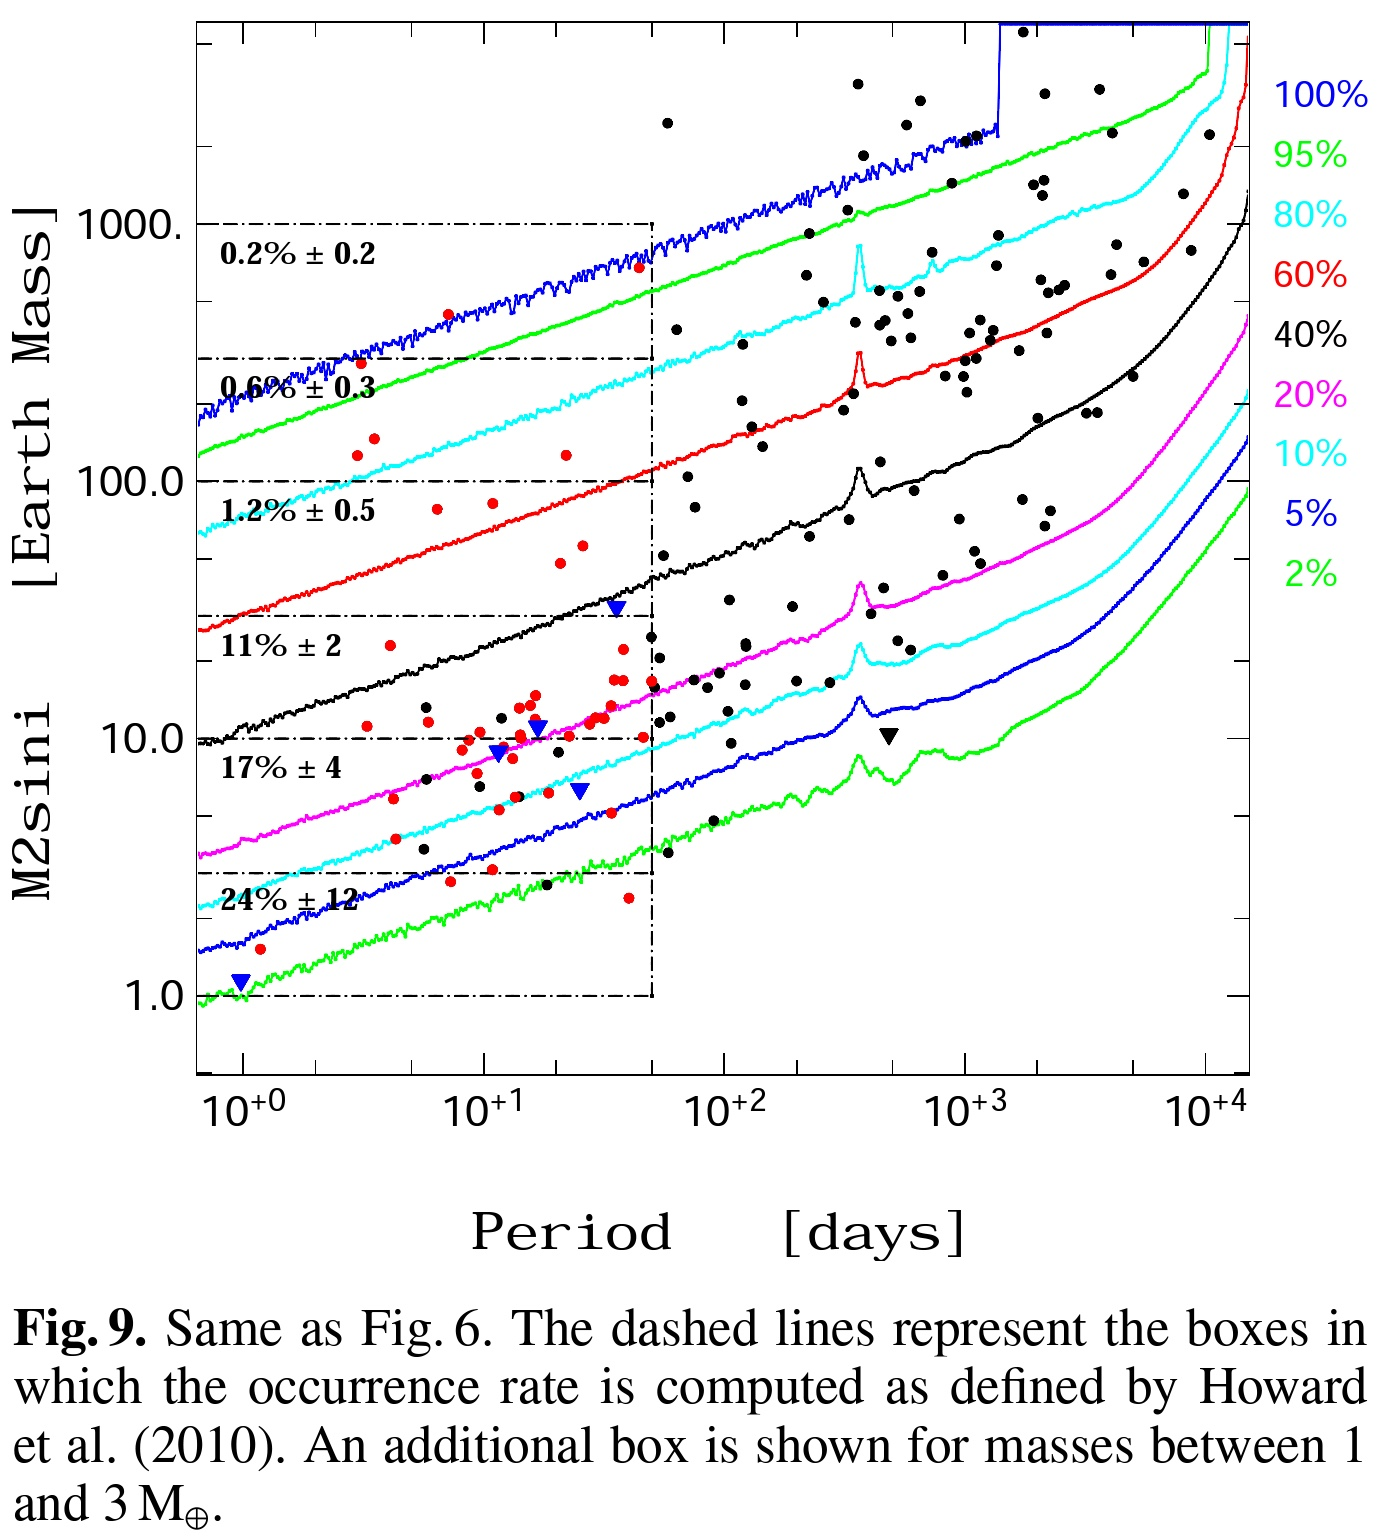
\includegraphics[trim={0cm 8cm 0 0},clip, width=0.99\textwidth]{PMfreq-short}\label{fig:PMfreq-short}
	\end{subfigure}
	\caption{Diagramma massa-periodo: frazione di stelle che ospitano pianeta con caratteristiche nella regione evidenziata. Da sinistra a destra: $P<10\si{\year}$ e $M>50\mearth{}$, $P<1\si{\year}$ e $M>3-100\mearth{}$, $P<50\si{\day}$ e $M=1-3/3-10/10-30/30-100/100-300/300-1000$. Da \cite{mayor2011harps}.}\label{fig:PMfreqs}
\end{figure}
\end{frame}

\begin{wordonframe}{RV survey: frequenze pianeti e bias osservativi}
Adesso passo a descrivere le propriet\'a degli esopianeti: una popolazione numerosa \'e stata osservata tramite osservazione della velocit\'a radiale della stella madre in una survey di 8 anni con lo spettrografo HARPS.
L'ampiezza della velocit\'a con cui la stella si muove \'e determinata dal periodo ($P$) e dalla massa del pianeta ($M_P$) oltre a fattori geometrici. (For Jupiter around the Sun ($a_J=5.2AU$, $P=11.9yr$: $K_J=\SI{12.5}{\meter\per\second}$))
Per tenere sotto controllo i bias osservativi si \'e scelto di fissare la probabilit\'a di rivelamento al $99\%$ e restringersi alle stelle che soddisfano la richiesta nella data regione del diagramma massa-distanza.
Le principali propriet\'a osservate sono massa del pianeta e periodo.
Pianeti gassosi con $M_P>50\mearth{}$, $P<\SI{10}{\year}$: $14\%$.
Pianeti gassosi con $100\mearth{}M_P>3\mearth{}$, $P<\SI{1}{\year}$: $47\%$.
Sistemi copatti con $P<\SI{50}{\day}$ e $M=1-3/3-10/10-30/30-100/100-300/300-1000$


Survey HARPS: radial velocity. La stella percorre ellisse attorno al CM stella-pianeta.
\begin{align*}
&v_r=\dot{z}=K[\cos{(\omega+\nu)}+e\cos{\omega}]\\
&K=\frac{2\pi}{P}\frac{a_*\sin{i}}{(1-e^2)\expy{1/2}}=(\frac{2\pi G}{P})\expy{1/3}\frac{M_p\sin{i}}{(M_p+M_*)\expy{2/3}}\frac{1}{(1-e^2)\expy{1/2}}
\end{align*}
$99\%$ detection threshold: $C(P,m\sin{i})$ frazione di stelle con sufficienti osservazioni per rivelare o escludere pianeta in data regione diagramma $(P,M)$, $N_{ij}=\frac{1}{C(P,M\sin{i})}$.
\end{wordonframe}

\begin{wordonframe}{Terza legge di Keplero}
	\begin{columns}[c]\begin{column}{0.7\textwidth}
			\begin{align*}
			&\ddvec{r}_1-\ddvec{r}_2=-\frac{G(m_1+m_2)}{|\vec{r}_1-\vec{r}_2|^3}(\vec{r}_1-\vec{r}_2)
			\end{align*}
		\end{column} \begin{column}{0.3\textwidth}
			\begin{align*}
			&P^2=\frac{4\pi^2}{G(m_1+m_2)}a^3
			\end{align*}
	\end{column}  \end{columns}
	\begin{columns}[c]\begin{column}{0.7\textwidth}
			\begin{align*}
			&m_1\vec{r}_1+m_2\vec{r}_2=0\\
			&\vec{r}_1-\vec{r}_2=\frac{m_1+m_2}{m_2}\vec{r}_1=-\frac{m_2+m_1}{m_1}\vec{r}_2\\
			&m_1\ddvec{r}_1=-Gm_1m_2\frac{m_2^3}{(m_1+m_2)^3r_1^3}\frac{m_1+m_2}{m_2}\vec{r}_1\\
			&\ddvec{r}_1=-\frac{\mu_1}{r_1^3}\vec{r}_1\\
			&\ddvec{r}_2=-\frac{\mu_2}{r_2^3}\vec{r}_2
			\end{align*}
		\end{column} \begin{column}{0.3\textwidth}
			\begin{align*}
			&P^2=\frac{4\pi^2}{\mu_1}a_1^3\\
			&P^2=\frac{4\pi^2}{\mu_2}a_2^3
			\end{align*}
	\end{column}  \end{columns}
\end{wordonframe}

\begin{frame}{HARPS: Distribuzione metallicit\'a}
\begin{figure}[!ht]
	\centering 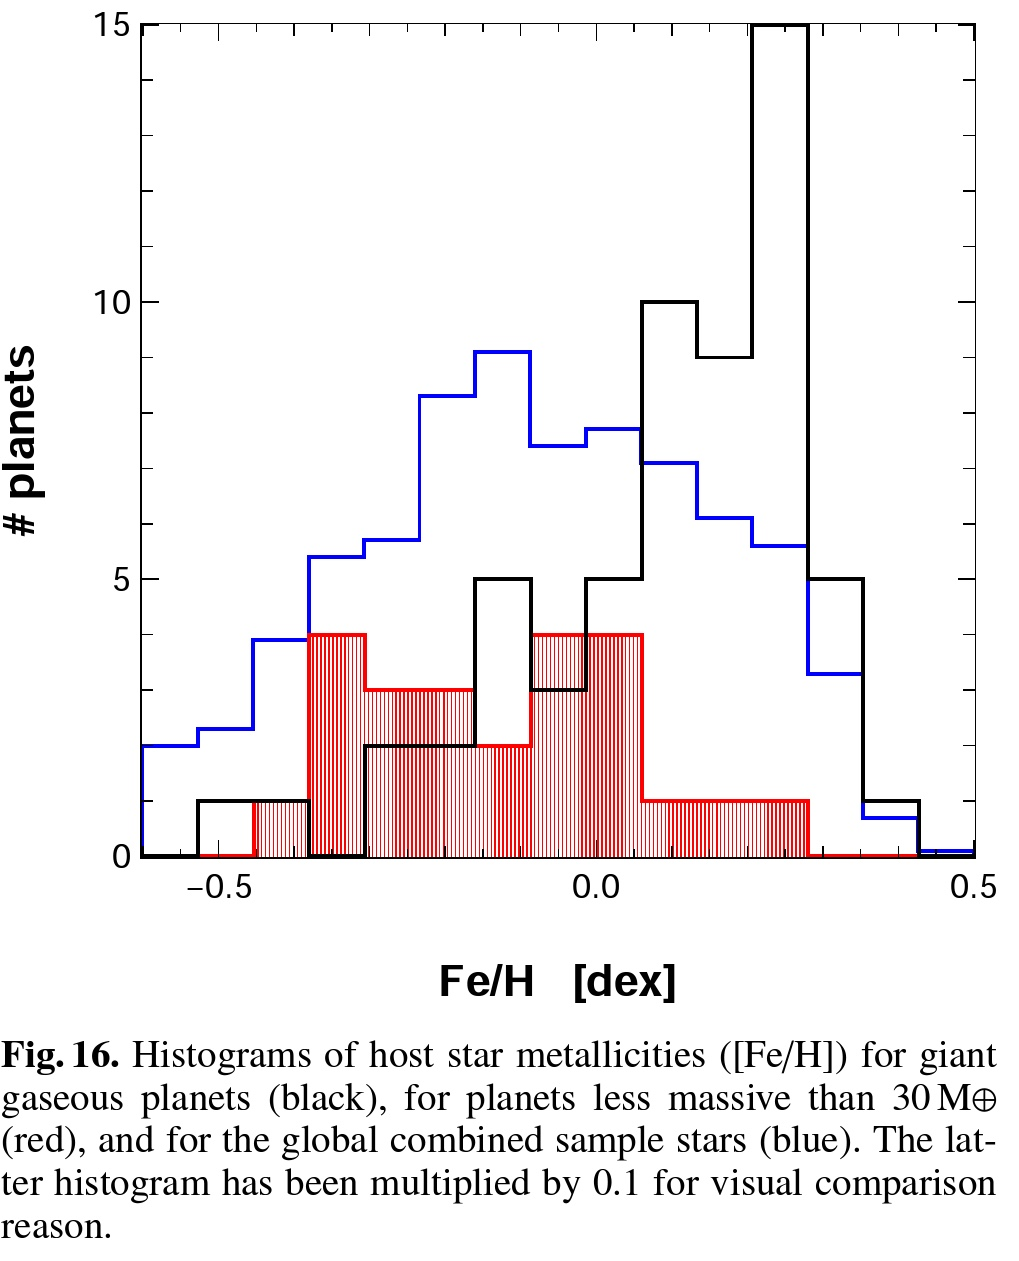
\includegraphics[trim={0cm 8cm 0 0},clip, width=0.53\textwidth]{PfreqvsFeH}
	\caption{Numero di pianeti in funzione della metallicit\'a stellare: nero dei giganti gassosi, rosso dei pianeti con $M\leq30\mearth{}$ e blu combinata. Da \cite{mayor2011harps}.}\label{fig:PfreqvsFeH}
\end{figure}
\end{frame}

\begin{wordonframe}{Harps: metallicit\'a-frequenza pianeti giganti}
La distribuzione dei pianeti con $M\geq30\mearth{}$ cresce con metallicit\'a stellare: il plot nero rappresenta il numero dei pianeti giganti ed \'e correlato con la metallicit\'a della stella.
Questa correlazione pu\'o apparire ovvia nello scenario di core accretion nel senso che maggiore metallicit\'a pu\'o portare prima a raggiungere la massa critica per accrescimento di gas.
\end{wordonframe}

\begin{frame}{HARPS: Distribuzione massa e periodo}
\begin{figure}[!ht]
	\begin{subfigure}[b]{0.45\textwidth} \centering 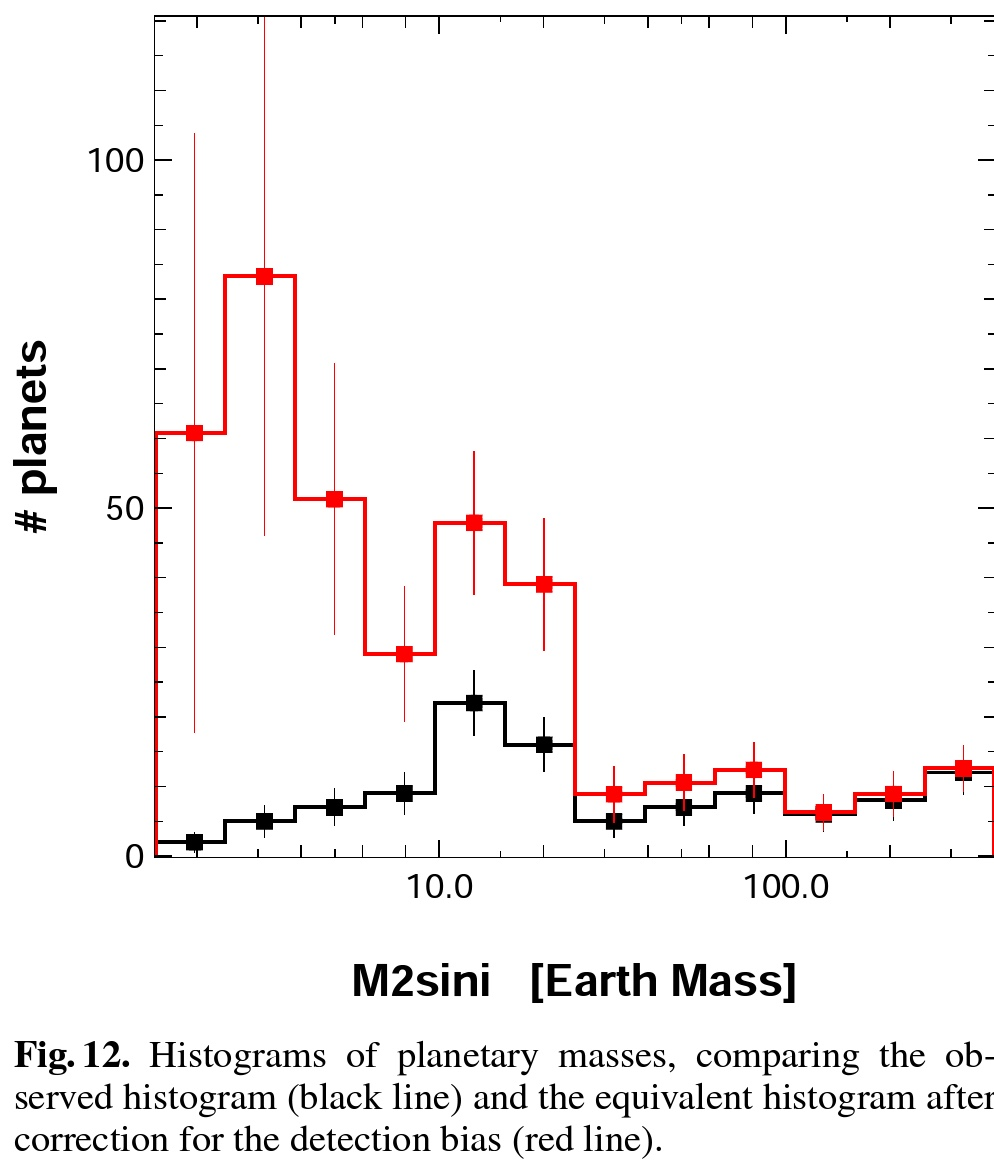
\includegraphics[trim={0cm 5cm 0 0},clip, width=0.94\textwidth]{freqvsM}
		\caption{Distribuzione di massa di massa dei pianeti: in rosso distribuzione corretta per bias osservativi. Da \cite{mayor2011harps}.}\label{fig:freqvsM} \end{subfigure}
	~
	\begin{subfigure}[b]{0.45\textwidth} \centering 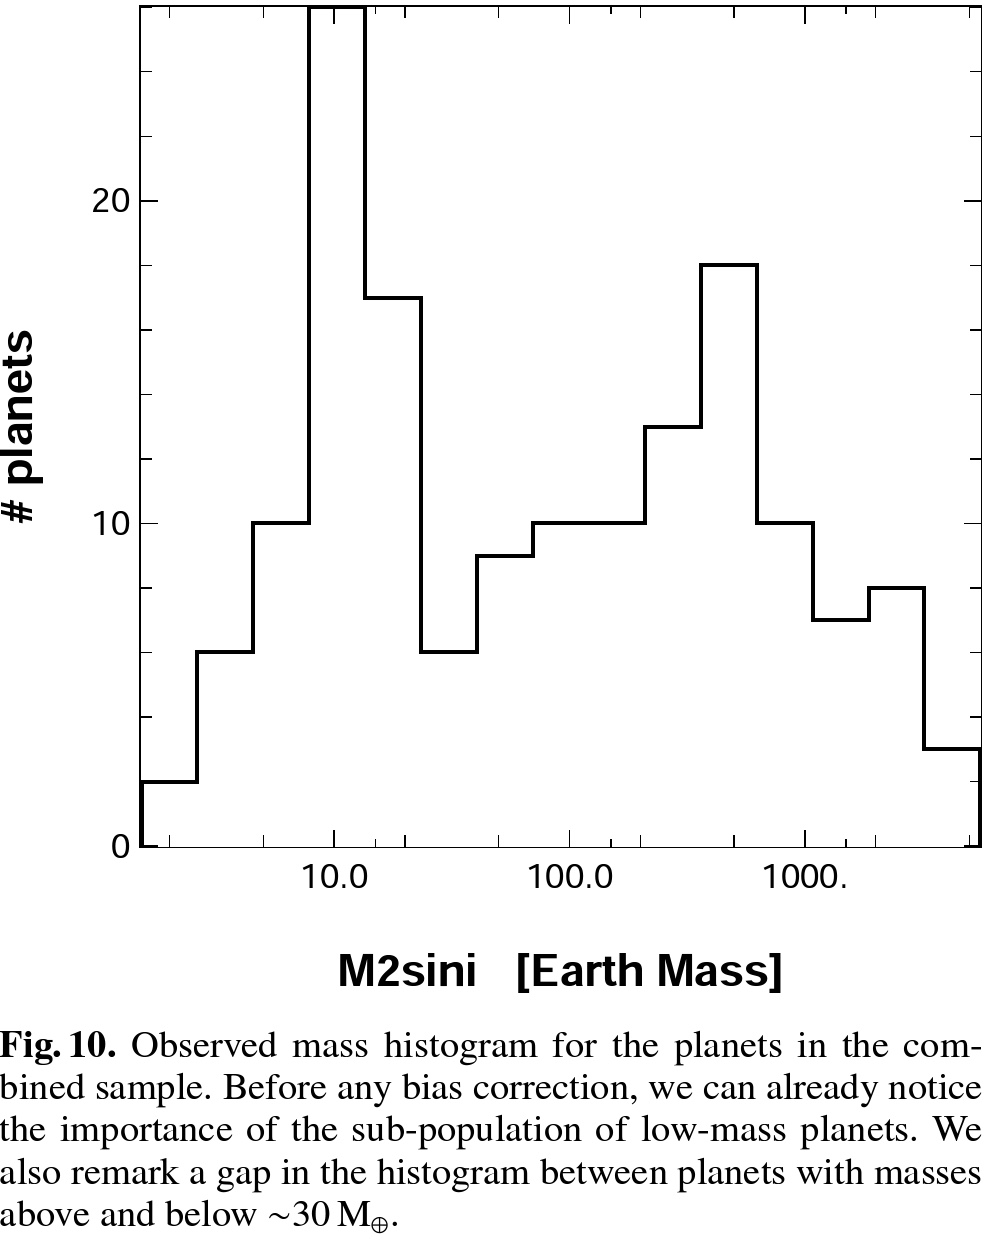
\includegraphics[trim={0cm 8cm 0 0},clip, width=0.94\textwidth]{freqvsMcomb}
		\caption{Distribuzione di massa dei pianeti osservata. Da \cite{mayor2011harps}.}\label{fig:freqvsMcomb}
	\end{subfigure}
\end{figure}
\end{frame}

\begin{wordonframe}{Harps: Distribuzione massa}
Massa: abbondanza pianeti di piccola massa: distribuzione crescente verso piccole masse e rapida diminuzione tra $\num{10}{30}\mearth{}$.
La distribuzione di massa mostra crescita per piccole masse e una rapida discesa tra \numrange{3}{10}$\mearth{}$: come vedremo la massa critica per accrescimento di gas \'e determinata dai modelli di formazione attorno a $10\mearth{}$.
Il picco nel regime dei pianeti giganti potrebbe essere dovuto ai pianeti che hanno accresciuto il gas nella fascia attorno all'orbita: rallentamento dell'accrescimento limitato dall'evoluzione viscosa del disco.
\end{wordonframe}

\begin{frame}{HARPS: Distribuzione periodo}
\begin{figure}[!ht]
\begin{subfigure}[b]{0.45\textwidth} \centering 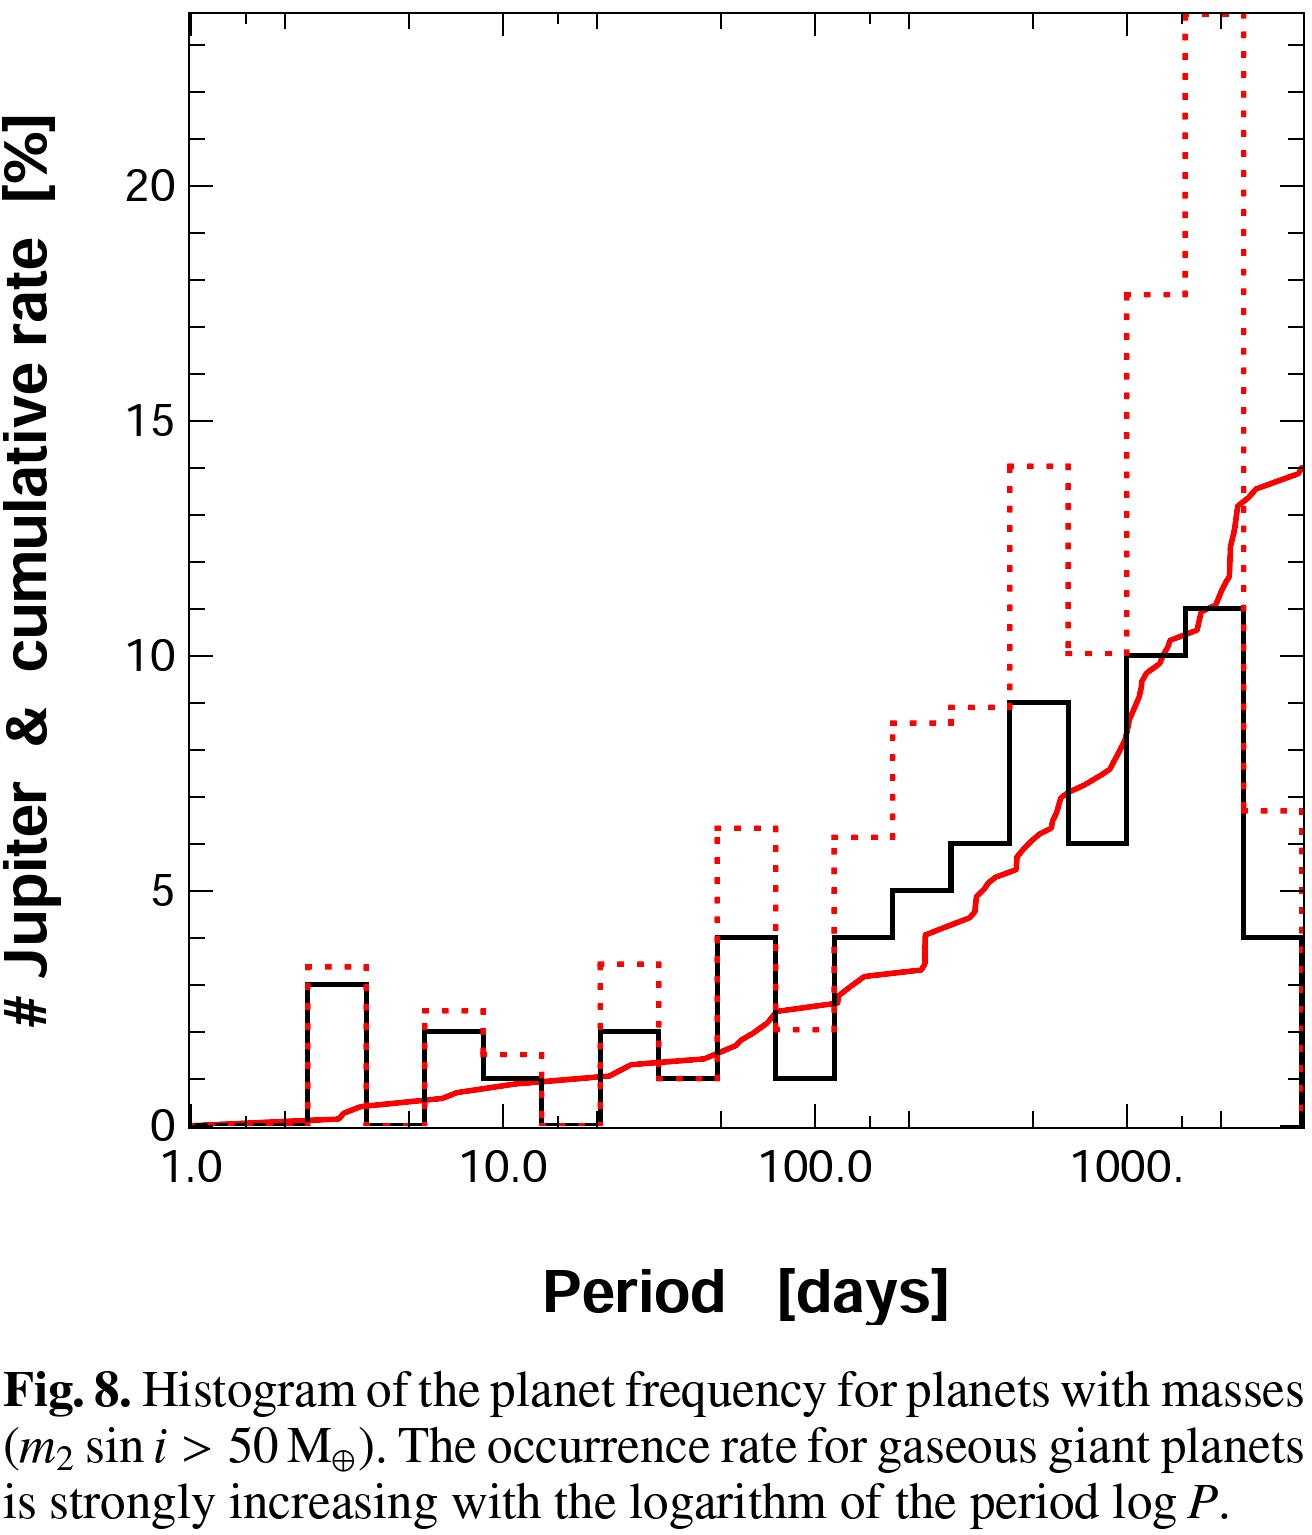
\includegraphics[trim={0cm 6cm 0 0},clip, width=0.98\textwidth]{freqvsPgiant}\caption{Frequenza pianeti con $M\geq 30\mearth{}$ in funzione del periodo orbitale; in rosso  tratteggiato con correzione bias osservativi. Da \cite{mayor2011harps}.}\label{fig:freqvsPgiant} \end{subfigure}
~
\begin{subfigure}[b]{0.45\textwidth} \centering 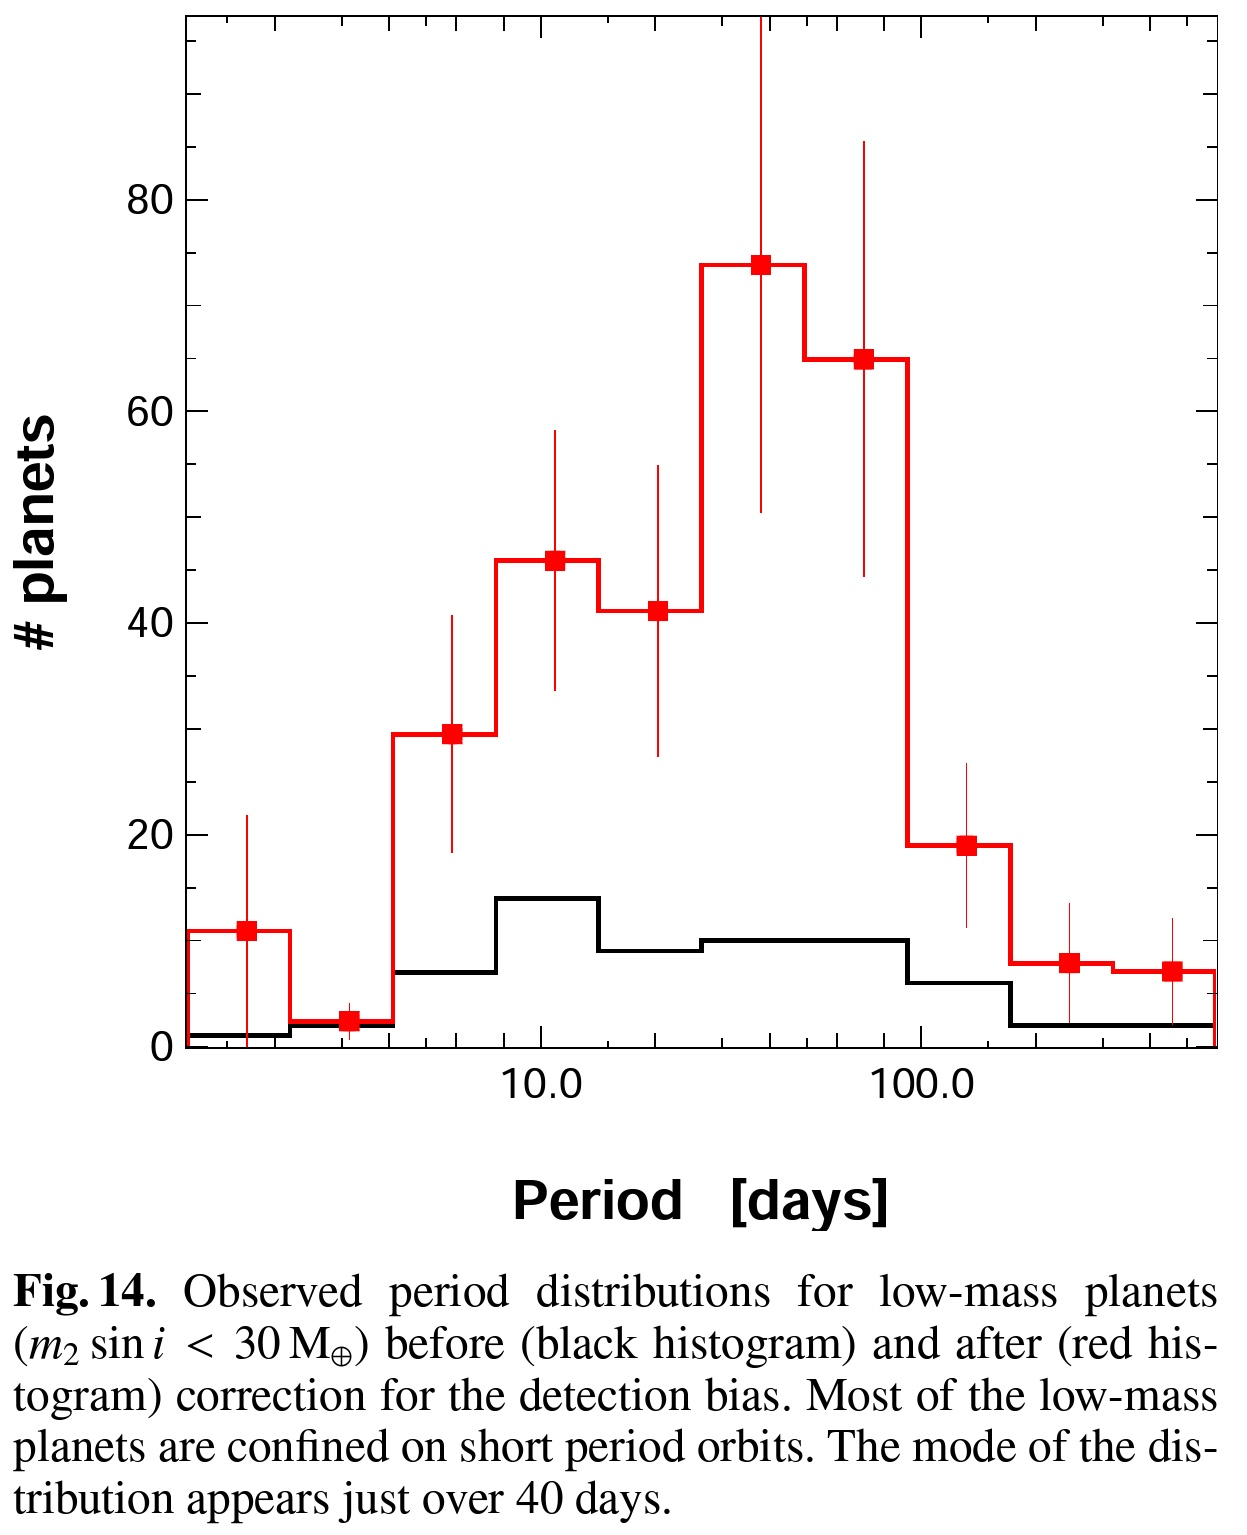
\includegraphics[trim={0cm 10cm 0 0},clip,width=0.98\textwidth]{freqvsPlowM} \caption{Frequenza pianeti con $M\leq 30\mearth{}$ in funzione del periodo orbitale; in rosso con correzione bias osservativi. Da \cite{mayor2011harps}.}\label{fig:freqvsPlowM}
\end{subfigure}
\end{figure}
\end{frame}

\begin{wordonframe}{Harps: Distribuzione periodo}
PAssiamo alla distribuzione dei periodi dove sono distinti i pianeti giganti $M_P>30\mearth{}$ e pianeti con $M_P<30\mearth{}$.
La frequenza dei pianeti giganti cresce con periodo fino a $P=\SI{1000}{\day}$. Pianeti di $M\leq30\mearth{}$ sono concentrati in sistemi compatti con $P=\SIrange{10}{100}{\day}$
\end{wordonframe}

\begin{frame}{Survey: kepler}
\begin{figure}[!ht]
	\begin{columns}[T]
\begin{column}{0.65\textwidth}
	\centering 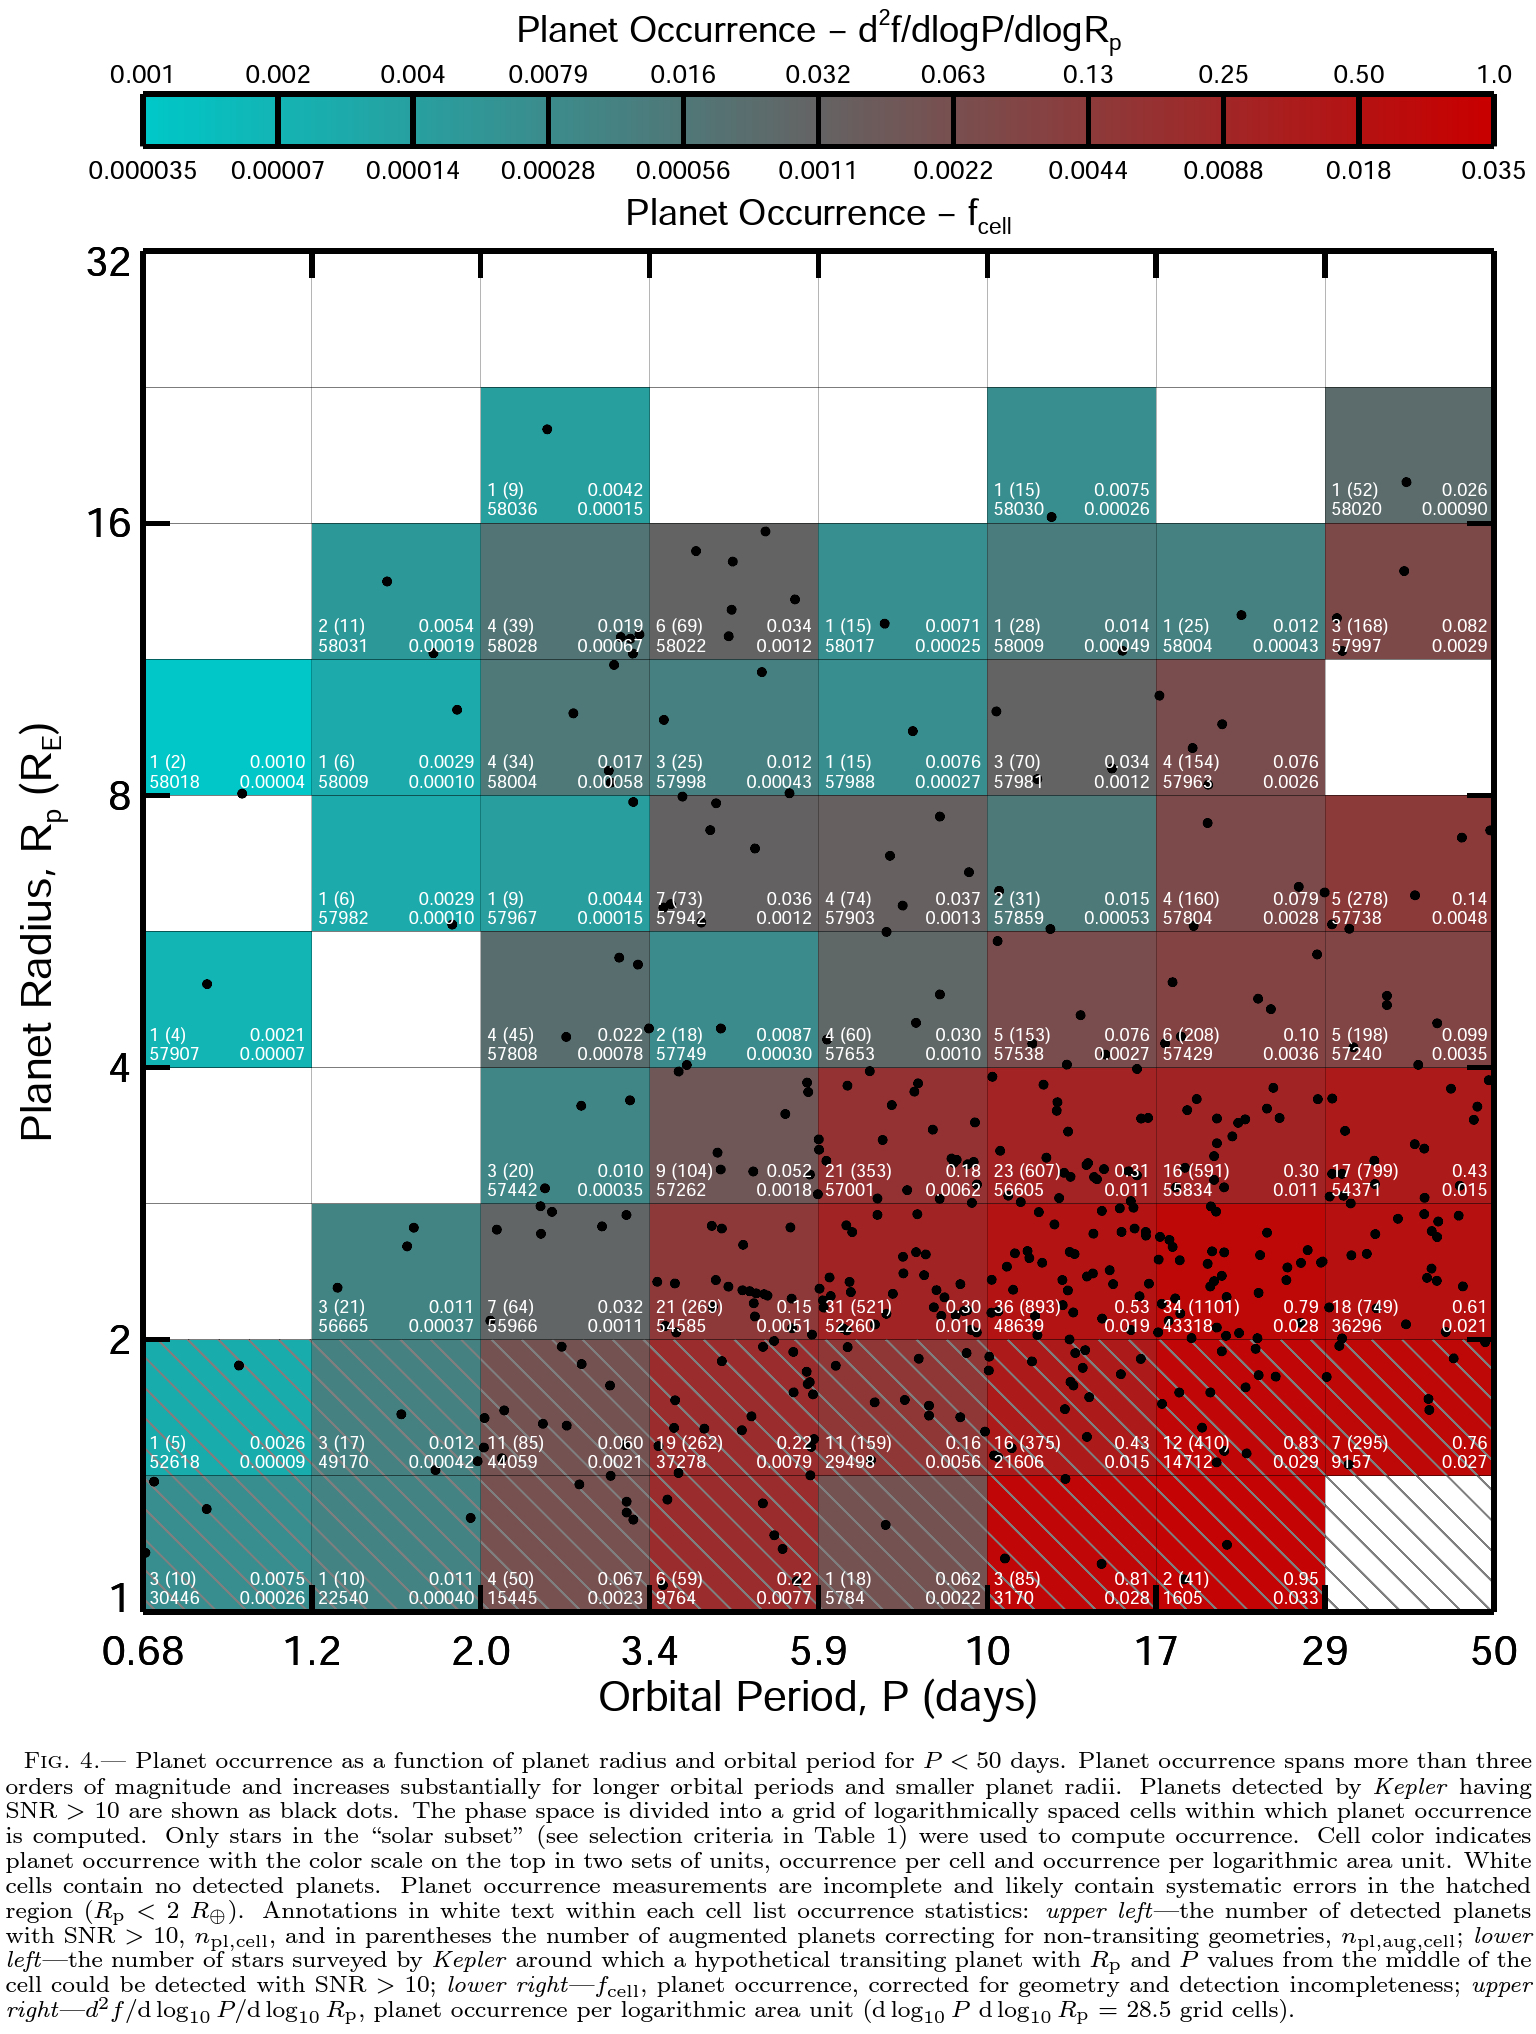
\includegraphics[trim={0cm 11cm 0 0},clip, width=0.9\textwidth]{keplerfreq}
\end{column}
\begin{column}{0.35\textwidth}
\caption{Pianeti con $\SNR{}>10$ nel diagramma $(P,R_P)$. Da \cite{howard2012planet}.}\label{fig:keplerfreq}
\end{column}
	\end{columns}

\end{figure}
\end{frame}

\begin{wordonframe}{Survey: kepler}
Un'altra tecnica osservativa che ha prodotto un abbondanti rivelamenti di pianeti \'e quella dei transiti. Le osservabili fondamentali sono la profondit\'a del transito $\Delta F\approx (R_P/R_*)^2$,cio'e la differenza relativa tra flusso non eclissato ed eclissato, i tempi di transito e il periodo. La probabilit\'a geometrica di transito \'e $\frac{R_*}{a}$ quindi \'e possibile osservare pianeti vicini alla stella. Ho considerato brevemente i risultati della survey eseguita con kepler di cui vediamo i risultati nel diagramma periodo-raggio.
Gli autori dimostrano la completezza delle osservazioni per pianeti con $P<\SI{50}{\day}$ (survey di 90 giorni) e $R_P<50\rearth{}$. In alto a sinistra in ogni cella sono riportati numero di pianeti osservati e la correzione per geometria di transito; mentre in alto a destra occorrenza di pianeti per unit\'a di area logaritmica.


La probabilit\'a che l'orbita di un pianeta sia allineata con l'osservatore in maniera da avere un transito \'e:
\begin{equation*}
p=(\frac{R_*\pm R_p}{a})(\frac{1}{1-e^2})
\end{equation*}
dove $\pm$ indica inclusione/esclusione di transiti a raso.
La maggiore probabilit\'a di transito per orbite eccentriche \'e compensata approssimativamente dalla minore probabilit\'a di rilevamento per la minor durata del transito.
In forma adimensionale l'equazione precedente si riscrive:
\begin{equation}
p=0.005(\frac{R_*}{\rsun{}})(\frac{a}{1AU})\expy{-1}(\frac{1}{1-e^2})
\end{equation}

$\SNR{}=\frac{\delta}{\sigma}\sqrt{\frac{n_{tr}t_{tr}}{\SI{3}{\hour}}}$
upper-left: $n_{pl,cell}(n_{pl,cell,aug})$, pianeti rivelati con $\SNR{}>10$ e correzione per probabilit\'a geometrica transito. Lower-left: stelle surveyed da kepler per cui un pianeta al centro della cella \'e rivelato con $\SNR{}>10$. Lower-right: $f_{cell}$ frequenza di pianeti corretta per probabilit\'a geometrica e incompletezza rivelamento. Upper-right: planet occurrence per logaritmic area unit.
\end{wordonframe}

\begin{frame}{Transiti: distribuzione raggi planetarii}
\begin{figure}[!ht]
	\begin{subfigure}[b]{0.47\textwidth}
		\centering
		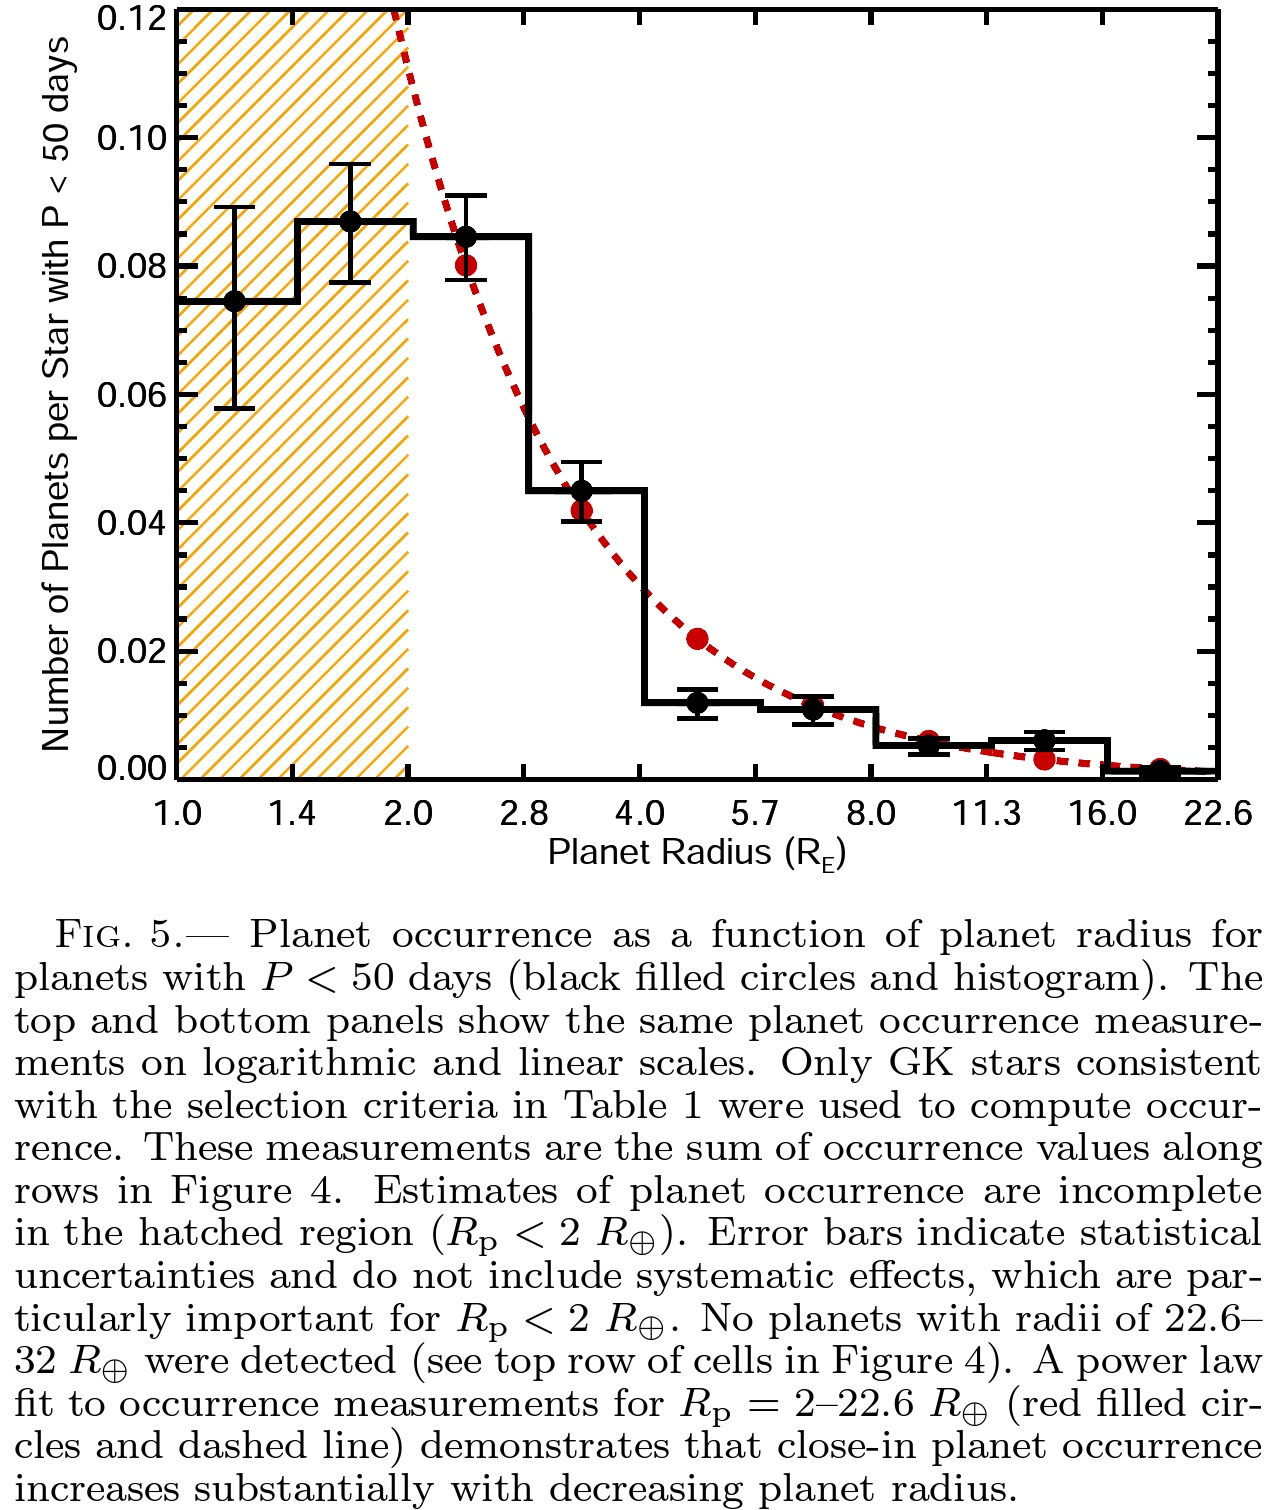
\includegraphics[trim={0cm 22cm 0 0},clip, width=0.95\textwidth]{freqvsRpl50d}
		\caption{Distribuzione raggi planetari: crescita esponenziale verso piccoli raggi. La regione barrata indica misure incomplete. Da \cite{howard2012planet}.}\label{fig:howard2012planet}
	\end{subfigure}
	~
	\begin{subfigure}[b]{0.49\textwidth} \centering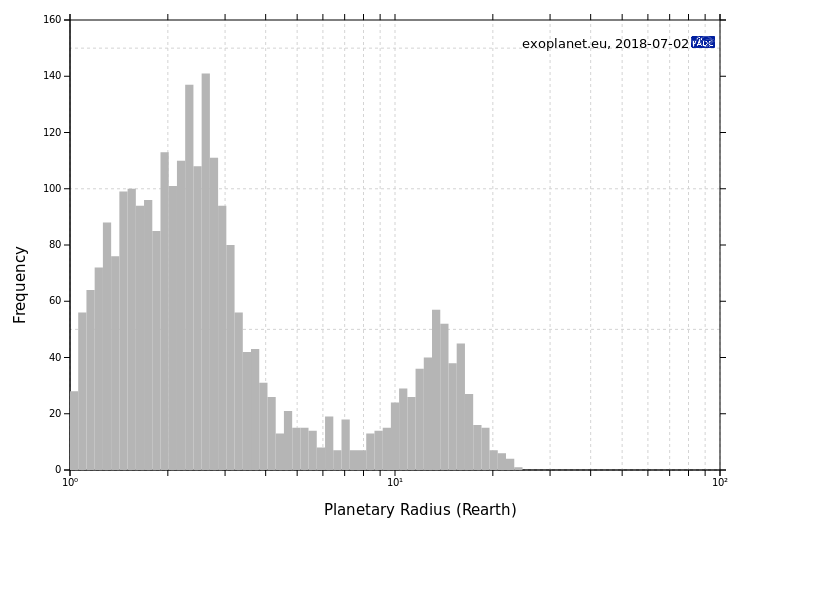
\includegraphics[trim={0cm 2.5cm 0 0},clip, keepaspectratio,width=0.9\textwidth]{Rfreq}\caption{Distribuzione radiale pianeti rivelati tramite T. Da \cite{exoplanet.eu} (luglio 2018): la frequenza ha andamento crescente verso pianeti di raggio terrestre, andamento piatto tra $4-10\rearth{}$ e picco a $R\approx\rjupiter{}$.}\label{fig:Rfreq}
	\end{subfigure}
\end{figure}
\end{frame}

\begin{wordonframe}{T: distribuzione raggi}
Cosa determina la distribuzione dei raggi?

\end{wordonframe}

\begin{frame}{Transiti: distribuzione raggi planetarii}
\begin{figure}[!ht]
	\centering 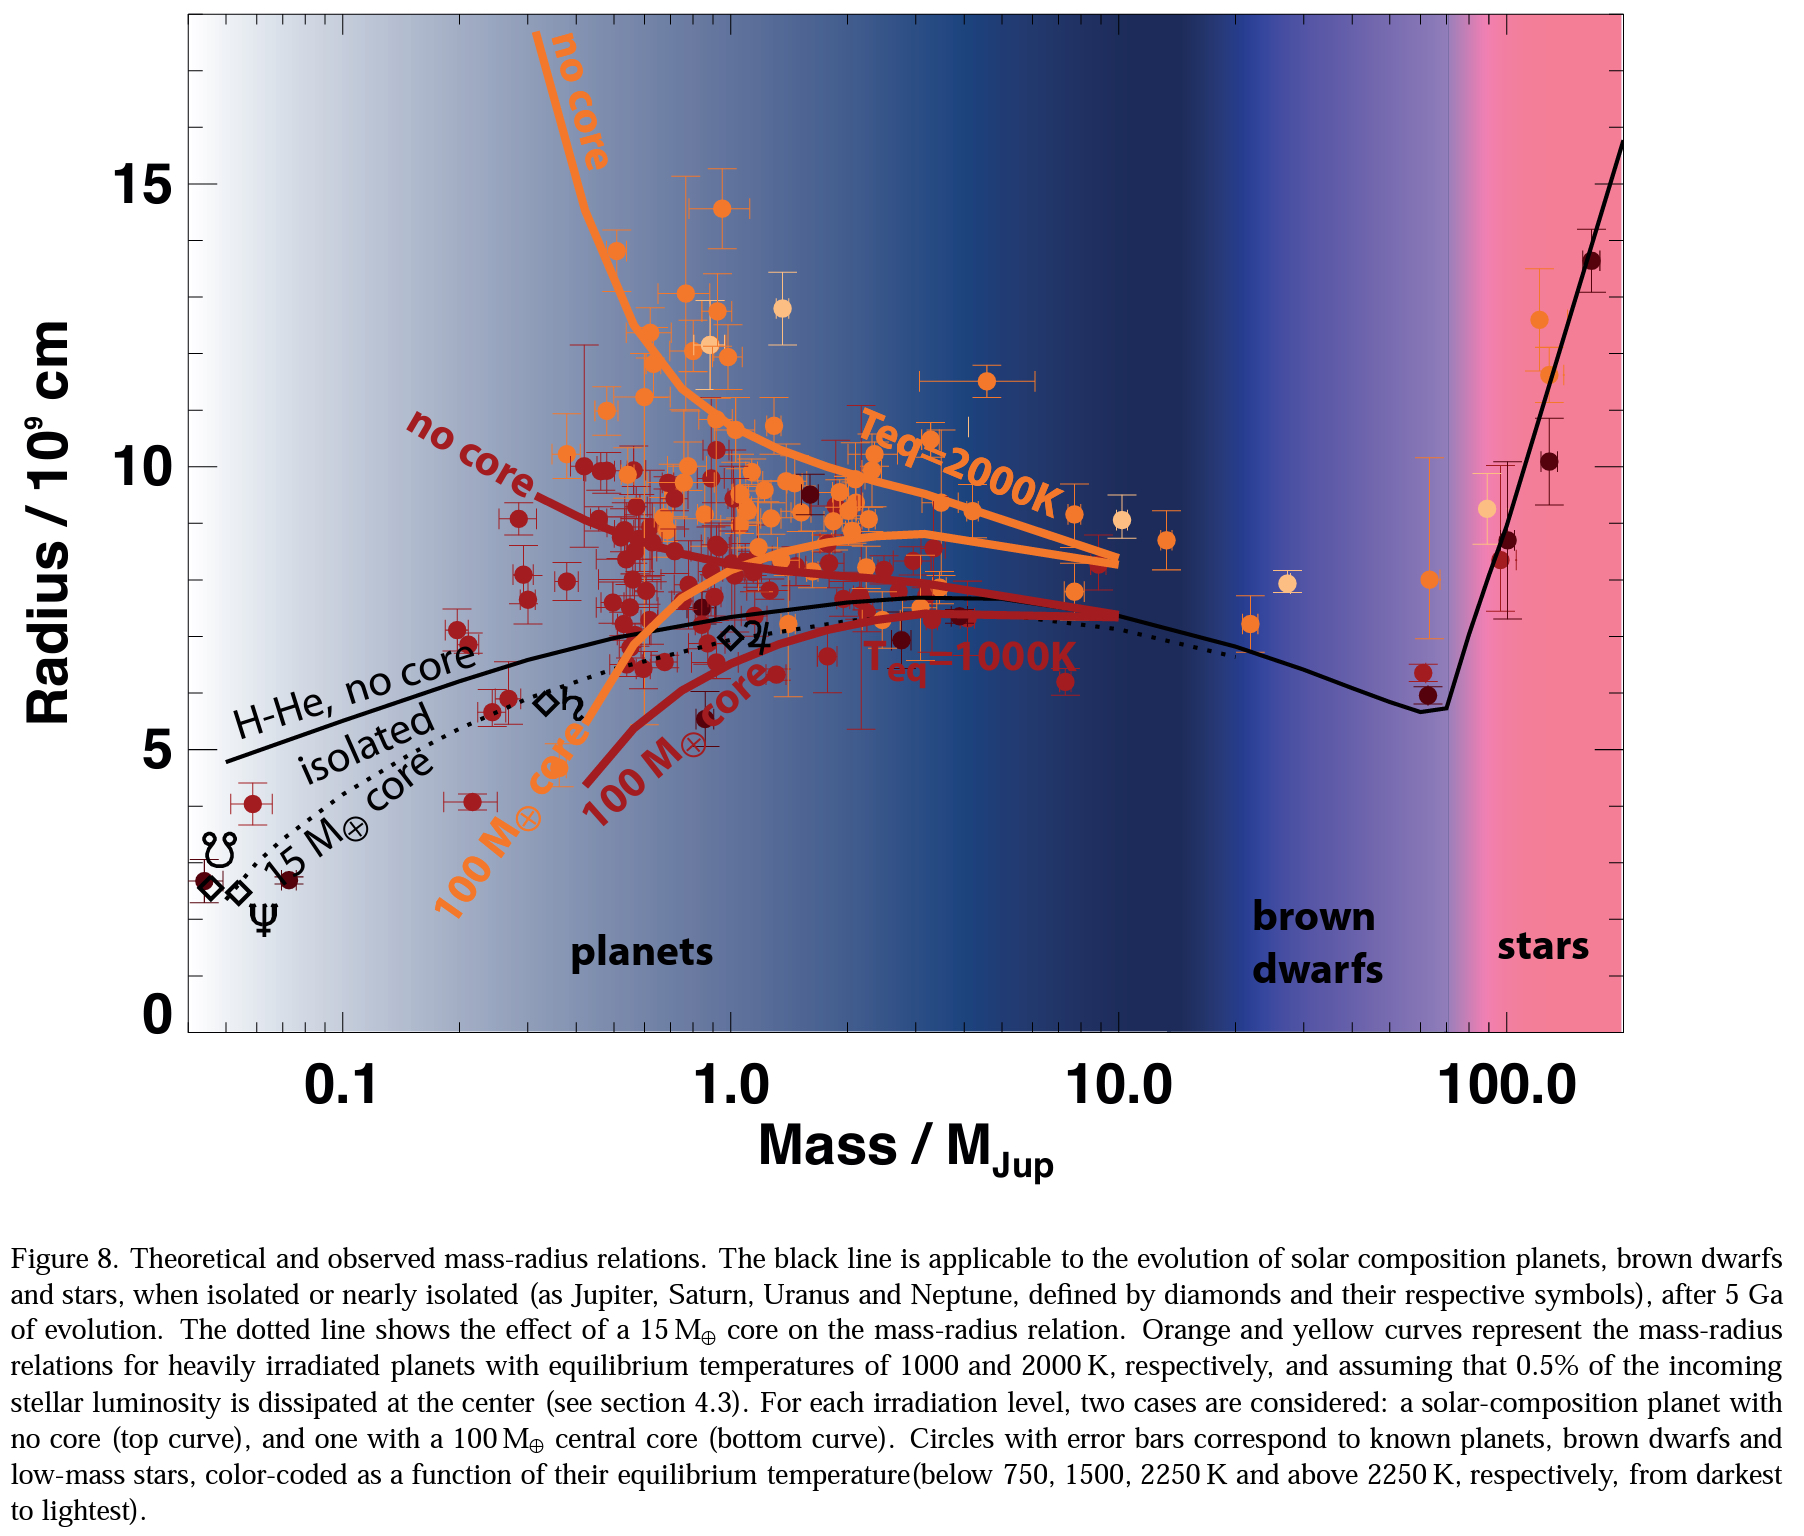
\includegraphics[trim={0cm 12cm 0 0},clip, width=0.8\textwidth]{MR-model-obs}
	\caption{Relazione massa-raggio determinata sulla base di modello planetario dopo \SI{5}{\giga\year}. Per gli esopianeti sono indicate le curve per temperature di equilibrio di \SI{1000}{\kelvin} e \SI{2500}{\kelvin}. Da \cite{guillot2014giant}.}\label{fig:MR-model-obs}
\end{figure}
\end{frame}

\begin{wordonframe}{Relazione massa-raggio}
Determino massa e raggio.
Relazione massa-raggio: 
La determinazione del raggio e massa permette di determinare la densit\'a media del pianeta.
La relazione massa-raggio dipende dalla composizione, che influenza la densit\'a e dall'equazione di stato che determina propriet\'a materia a alte pressioni (compressibilit\'a) e bilancio termico.
consiste in $R\propto M\expy{1/3}$ nella parte incompressibile, $R$indipendente da $M$ per raggi gioviani fino al regime tipico della materia degenere $R\propto M\expy{-1/3}$ nella regione delle brown dwarf.
\end{wordonframe}